\part{Geometría analítica}

\null\vfill
\begin{Huge}\begin{center}
III. Geometria Analítica	
\end{center}\end{Huge}

\vspace{1.5cm}

\begin{figure}[H]
	\centering
	\includegraphics[width=.9\textwidth]{imagenes/part3.png}	
\end{figure}
\par
\vfill

\chapter{Vectores en el plano. Producto Escalar}

\begin{tikzpicture}
	\fill [left color=red!50, right color=teal!50] (0,0) rectangle (6.5,.2);
	\fill [left color=teal!50, right color=blue!50] (6.5,0) rectangle (11.5,.2);
	\end{tikzpicture}
	
	
	
\vspace{15mm}


\begin{adjustwidth}{40pt}{40pt}
\begin{cuadro-gris}

	\begin{multicols}{2}
	$\triangleright \quad$  Vectores 2-D.
	
	$\triangleright \quad$  Operaciones con vectores.
	
	$\triangleright \quad$  Base.
	
	$\triangleright \quad$  Producto escalar.
	\end{multicols}
	
\end{cuadro-gris}
\end{adjustwidth}



\vspace{5mm}
\section{Vectores}

\begin{tikzpicture}
	\fill [left color=red!50, right color=teal!50] (0,0) rectangle (3.5,.1);
	\fill [left color=teal!50, right color=blue!50] (3.5,0) rectangle (7.5,.1);
	\end{tikzpicture}
\vspace{0.5cm}	
	
	
Una magnitud física es toda aquella propiedad de un cuerpo que puede ser medida. La masa, el volumen, la velocidad o la temperatura son magnitudes físicas. El aroma o la simpatía, puesto que no pueden medirse, no son magnitudes físicas.

Para muchas magnitudes físicas, basta con indicar su valor para que estén perfectamente definidas. Así, por ejemplo, si decimos que determinada persona tiene una temperatura de 38$^o$ C, sabemos perfectamente que tiene fiebre y si otra mide 145 cm de altura está claro que es bajita. Cuando una magnitud queda definida por su valor, un número acompañado de una unidad, recibe el nombre de \emph{magnitud escalar}.

Otras magnitudes, con su valor numérico, no nos suministran toda la información. Así si nos dicen que hay un viento de 50 km/h apenas sabemos algo más que al principio. Deberían informarnos también desde donde sopla y hacia donde se dirige. Estas magnitudes que, además de un valor numérico, se describen señalando también una dirección y un sentido se llaman \emph{magnitudes vectoriales} y se representan mediante vectores. Podemos visualizar un vector (en el plano o en el espacio tridimensional) como un segmento de recta dirigido o una flecha

Así cada vector quedará identificado por tres características fundamentales: módulo o longitud, dirección y sentido.	
	
	
\begin{definition}[ Vector]

Vector: segmento orientado, de origen $A$ y extremo $B$, lo denotaremos por $\ \vec v=\overrightarrow {AB}$
\begin{multicols}{2}

\vspace{2mm} $\bullet \ $ Módulo de un vector es la longitud del segmento que lo representa, $\ |\vec v|=d(A,B)$



\vspace{2mm} $\bullet \ $ Dirección de un vector es la recta a la cual pertenece, $\ r \, , \  $ o cualquier recta paralela a ésta.

\vspace{2mm} $\bullet \ $ Sentido de un vector está dado por la orientación del segmento que lo representa, desde $A$ hacia $B$, el sentido  lo determina la punta de la flecha.	\begin{small}{ (Una dirección tiene dos sentidos, se les llama sentidos `contrarios')} \end{small}


\begin{figure}[H]
	\centering
	\includegraphics[width=.5\textwidth]{img-vec/vec01.png}	
\end{figure}
\end{multicols}

\end{definition}

\underline{Vectores iguales}: dos vectores son iguales cuando tienen el mismo módulo, dirección y sentido (aunque difieran en su posición, es decir, en sus punto de aplicación). También se les suele llamar \emph{vectores equipolentes}.
\textcolor{gris}{Por lo tanto, si dos vectores se diferencian en cualquiera de los tres elementos (módulo, dirección o sentido) los consideraremos distintos.}
\begin{multicols}{2}
Todos los vectores equipolentes a uno dado forman lo que llamaremos \textbf{\emph{vector libre}}. De otro modo, los vectores en matemáticas se pueden desplazar paralelamente a sí mismos por todo el plano, han de conservar módulo (tamaño), dirección (estar en rectas paralelas) y sentido (el que da la flecha).

Cuando se quiere usar un vector en un punto tomamos aquel vector equipolente que tiene origen en ese punto, tendremos un \emph{vector fijo}, hemos fijado un representante del vector libre.
\begin{figure}[H]
	\centering
	\includegraphics[width=.5\textwidth]{img-vec/vec02.png}	
\end{figure}

\end{multicols}
	
\begin{multicols}{2}
Un punto en el plano no es más que una posición. Se representan por letras mayúsculas del alfabeto latino. El punto $P(2,1)$ está 2 unidades a la derecha de origen y 1 hacia arriba.

Por contra, un 	\underline{vector representa un movimiento}, así, el vector $\vec v=(2,3)$ significa un desplazamiento de 2 unidades a la derecha y 3 hacia arriba.
\begin{figure}[H]
	\centering
	\includegraphics[width=.3\textwidth]{img-vec/vec03.png}	
\end{figure}	
\end{multicols}
	
Los vectores desplazan puntos: $\ \ P+\vec v = Q\, : \quad (2,1)+(2,3)=(4,4)$	
\vspace{3mm}%%%%%%%%%	
\begin{figure}[H]
	\centering
	\includegraphics[width=.5\textwidth]{img-vec/vec14.jpeg}	
\end{figure}
	
	
%\vspace{3mm}%%%%%%%%%
\section{Operaciones con vectores}

\begin{tikzpicture}
	\fill [left color=red!50, right color=teal!50] (0,0) rectangle (3.5,.1);
	\fill [left color=teal!50, right color=blue!50] (3.5,0) rectangle (7.5,.1);
	\end{tikzpicture}
\vspace{0.5cm}		
	
\textbf{Producto de un vector por un escalar} (por un número) \footnote{ No confundir `producto por un escalar' con `producto escalar', que se definirá más adelante.}

$\triangleright \ $ El producto de un número real $k$ por un vector $\vec v$ es un vector $k\, \vec v$ que tiene:
\begin{multicols}{2}
\begin{itemize}
\item por módulo, $|k|\ |\vec v|$
\item dirección, la de $\vec v$
\item sentido $\ \begin{cases}	 \ \text{el mismo que } \vec v & \text{si } k>0 \\ \ \text{contrario a } \vec v & \text{si } k<0 \end{cases}$
\end{itemize}
\begin{figure}[H]
	\centering
	\includegraphics[width=.3\textwidth]{img-vec/vec05.png}	
\end{figure}
\end{multicols}

\textbf{Suma de vectores}

$\triangleright \ $ Método del paralelogramo para la suma de vectores:

Dados dos vectores $\vec a$ y $\vec b$, para sumarlos debemos considerar dos vectores iguales a los dados que se unen en su origen. Luego se dibuja un paralelogramo que tiene a ambos vectores como lados adyacentes, siendo la diagonal, del paralelogramo, la dirección del vector suma, cuyo origen coincide con el origen de los dos vectores.

$\triangleright \ $ Método del polígono para la suma de vectores (vectores consecutivos)

Dados dos vectores  $\vec a$ y $\vec b$, para sumarlos debemos considerar dos vectores iguales a los dados en que el segundo vector empieza donde acaba el primero (consecutivos). El vector resultante tiene como origen el punto de partida del primero y como extremo el extremo del último vector.

\begin{figure}[H]
	\centering
	\includegraphics[width=1\textwidth]{img-vec/vec04.png}	
\end{figure}


\underline{Observaciones}
\begin{itemize}
\item  $\subrayado{ \text{si } \  \vec u = k\, \vec v \ \leftrightarrow \ \vec u \parallel \vec v }$
\item resta de vectores: $\quad \subrayado{\vec u - \vec v \ = \  	\vec u + (-1)\, \vec v}$
\end{itemize}

\begin{theorem}[ Propiedades del producto por un escalar y de la suma de vectores]

\begin{enumerate}
\item $\vec u + \vec v=\vec v+\vec u\ $ (conmutativa)
\item $\vec u + (\vec v + \vec w)=(\vec u + \vec v) + \vec w = \vec u + \vec v + \vec w \ $ (asociativa)	
\item $\vec 0 + \vec u = \vec u \ $ ($\vec 0$ neutro)
\item $(1-)\, \vec u = -\vec u\ $ (opuesto)
\item $k(\vec u+\vec v)=k\vec u +k\vec v;\qquad (k_1+k_2)\vec u=k_1 \vec u+k_2 \vec v;\qquad (k_1\, k_2)\, \vec u=k_1\, (k_2\, \vec u)$
\item $1\, \vec u = \vec u; \qquad 0\, \vec u =\vec 0$
\end{enumerate}	
\end{theorem}

\vspace{5mm}

\begin{miejemplo}

En el hexágono de la figura, sean los vectores $\ \overrightarrow{AB} = \vec u \ $ y $\ \overrightarrow{AC} = \vec v \ $, expresa como combinación lineal de los los vectores:
\begin{multicols}{2}

\vspace{2mm}$\overrightarrow{BC};\quad \overrightarrow{AO};\quad \overrightarrow{AD};\quad \overrightarrow{DO};\quad \overrightarrow{CD};\quad \overrightarrow{AE}$

\vspace{4mm} $\overrightarrow{BC}=-\vec u + \vec v$

\vspace{2mm} $\overrightarrow{AO}=\overrightarrow{BC}=-\vec u + \vec v$

\vspace{2mm} $\overrightarrow{AD}=2\overrightarrow{AO}=-2\vec u + 2\vec v$

\vspace{2mm} $\overrightarrow{DO}=-\overrightarrow{BC}=\vec u - \vec v$

\vspace{2mm} $\overrightarrow{CD}=\overrightarrow{CA}+\overrightarrow{AD}=-\vec v +(-2\vec u+2 \vec v)=-2\vec u+\vec v$

\vspace{2mm} $\overrightarrow{AE}=\overrightarrow{AD}+\overrightarrow{DE}=-(-2\vec u+2 \vec v)-\vec u=-3\vec u+2\vec v$
\begin{figure}[H]
	\centering
	\includegraphics[width=0.4\textwidth]{img-vec/vec08.png}	
\end{figure}	
\end{multicols}
\end{miejemplo}

\vspace{5mm}
\section{Base}

\begin{tikzpicture}
	\fill [left color=red!50, right color=teal!50] (0,0) rectangle (3.5,.1);
	\fill [left color=teal!50, right color=blue!50] (3.5,0) rectangle (7.5,.1);
	\end{tikzpicture}
\vspace{0.5cm}	

	
	
\begin{definition}[ Combinación lineal]

Dados dos vectores $\ \vec u \ \text{ y } \ \vec v \ $ y dos números reales $\ \alpha \  \text{ y } \ \beta \, , \  $ se llama \emph{combinación lineal} de estos vectores a la expresión: $\ \ \boldsymbol{\alpha \, \vec u \ + \ \beta \, \vec v }$
	
\end{definition}
\vspace{5mm}
\begin{definition}[ Base]

Dos vectores $\ \vec u \ \text{ y } \ \vec v \ $ de distinta dirección forman una \textbf{\emph{Base}}, es decir, cualquier otro vector $\ \vec w \ $ se puede escribir de forma única como combinación lineal de los vectores de la base:

$$\mathcal B=\{\vec u,\vec v\} \, : \quad \forall \vec w \  \exists! \,  \alpha, \ \wedge\  \exists! \,  \beta \in \mathbb R \ / \quad \vec w \ = \alpha \, \vec u \ + \ \beta \, \vec v $$

Los números $\ \alpha \  \text{ y } \ \beta \, , \  $ escritos en forma de par ordenado, $\ (\alpha,\beta)\ $ son las \textbf{\emph{componentes}} del vector $\ \vec w\ $ en la base $\ \mathcal B=\{\vec u,\vec v\}\ $
\end{definition}

\begin{multicols}{2}

Dispuesto $\vec u$ y $\vec v$ unidos por sus extremos, dibujamos $\vec w$ también con el extremos común a los anteriores.

Prolongamos las rectas que definen los vectores de la base $\vec u$ y $\vec v$ y, desde el extremo de $\vec w$ trazamos rectas paralelas a las anteriores hasta cortarlas.

Estas intersecciones determinan los vectores $\vec u'$ y $\vec v'$ que, al tener la misma dirección que $\vec u$ y $\vec v$ se pueden expresar como $\vec u'=2\vec v$ y $\vec v'=3\vec v$, coeficientes que serán las componentes del vector $\vec w$ en la base $\mathcal B=\{\vec u,\vec v\}$

\begin{figure}[H]
	\centering
	\includegraphics[width=0.5\textwidth]{img-vec/vec06.png}	
\end{figure}	
\end{multicols}

\vspace{5mm}

\underline{Observación}: un vector se escribe de forma única en una base. En otra base, este mismo vector se escribirá de manera distinta.

En la figura siguiente,  $\ \vec w \ = \ (5,11)_{B\{\vec u_1,\vec u_2\}} = \ (-6,8)_{B\{\vec v_1,\vec V_2\}}$


\begin{figure}[H]
	\centering
	\includegraphics[width=0.95\textwidth]{img-vec/vec07.png}	
\end{figure}


\color{gris}
\rule{300pt}{0.1pt}

\underline{Analíticamente}: Sea $\mathcal B=\{\vec u_1,\vec u_2\}$ y $\mathcal B'=\{\vec v_1,\vec v_2\}$, tenemos que $\vec w_{\mathcal B}=(5,11)$ y $\vec w_{\mathcal B'}=(-6,8)$.

Veamos como se escriben cada uno de los vectores de $\mathcal B'$ en la base $\mathcal B$:

De la figura: $\ \vec v_1=\dfrac 1 2 (\vec u_1-\vec u_2)=\dfrac 1 2 \vec u_1-\dfrac 1 2u_2\, ; \qquad \vec v_2=\vec u_1+\vec u_2\, , \ $ entonces

$\vec w_{\mathcal B'}=(-6,8)_{\mathcal B'}=-6\vec v_1+8\vec v_2= -6 \left( \dfrac 1 2 \vec u_1-\dfrac 1 2u_2 \right) \ + \ 8 (\vec u_1+\vec u_2)=-3\vec u_1+3\vec u_2+8\vec u_1+8\vec u_2=5\vec u_1+11\vec u_2=(5,11)_{\mathcal B}=\vec w_{\mathcal B}$

\vspace{-7mm} \begin{flushright} \rule{300pt}{0.1pt} \end{flushright}
 
\color{black}

\vspace{5mm}

\begin{definition}[ BON]

Decimos que la base $\ B=\{\vec u_1, \vec u_2\} \ $ es una \emph{base orto-normal}, BON, si:

$$\vec u \perp \vec v \quad \wedge \quad |\vec u|=|\vec v|=1 $$	


\begin{multicols}{2}
\textbf{\emph{Base canónica}} es una BON establecida por un canon, regla, norma o modelo: tomamos en el plano cuadrículas de lado unidad. La forman los vectores que denominaremos $\ \boldsymbol {\vec i} \ $ (en ej eje X) y  $\ \boldsymbol {\vec j} \ $ (en el eje Y)
\begin{figure}[H]
	\centering
	\includegraphics[width=0.25\textwidth]{img-vec/vec09.png}	
\end{figure}
\end{multicols}
\end{definition}

\underline{Observación}: los \underline{puntos} se definen por 	\underline{\emph{coordenadas}}, son fijos y en su descripción no pondremos el signo igual, $P(1,3)$. Los \underline{vectores} se definen por sus \underline{\emph{componentes}}, elegida una base, son móviles y para describirlos usaremos una flechita encima y las componentes precedidas del signo igual, $\vec u=(3,2)$

\vspace{0.5cm}

\subsection{Operaciones en componentes}
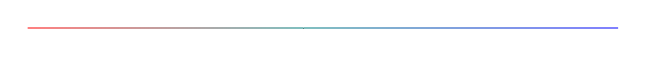
\begin{tikzpicture}
	\fill [left color=red!50, right color=teal!50] (0,0) rectangle (3.5,.01);
	\fill [left color=teal!50, right color=blue!50] (3.5,0) rectangle (7.5,.01);
	\end{tikzpicture}
\vspace{0.5cm}

Sean $\ \alpha, \, \beta \, \in \mathbb R\ $ dos números reales y $\ \vec u, \ \vec vº $ dos vectores libres del plano cuyas componentes, elegida una base $\ \mathcal B=\{\vec e_1, \vec e_2\} \ $ son $\ \vec u=(u_1,u_2)\ $ y $\ \vec v=(v_1,v_2)\, , \  $ entonces

\vspace{-5mm}
$$\subrayado{\boldsymbol{ k\cdot \vec u  } \ = }\ k \cdot (u_1,u_2) \ \subrayado{ = \  \boldsymbol{(k\, u_1\, , \ k\, u_2)} } \qquad \qquad \subrayado{\boldsymbol{\vec u + \vec v} \ =} \ (u_1,u_2)+(v_1,v_2)\ \subrayado{ = \ \boldsymbol{(u_1+v_1,u_2+v_2)} }$$


\begin{miejemplo}

Si en una determinada base las componentes de dos vectores son $\vec u=(2,-3)$ y $\vec v=(-3,4)$, calcula las componentes de $2\vec u-3\vec v$

\vspace{5mm} $2\vec u-3\vec v=2(2,-3)-3(-3,4)=(4,-6)-(-9,12)=(-5,-18)$	
\end{miejemplo}

\vspace{5mm}
\begin{miejemplo}

\begin{figure}[H]
	\centering
	\includegraphics[width=0.9\textwidth]{img-vec/vec10.png}	
\end{figure}

\vspace{-5mm} Operaciones en componentes $\quad \frac 12 \vec v=\frac 12 (3,1)=(3/2,1/2) \quad \vec u+\vec v=(1,2)+(3,1)=(4,3)$
	
\end{miejemplo}




\vspace{5mm}

En el plano, elegido un punto como origen, $\mathcal O$, se ubican partiendo de el los vectores de la base elegida, $\mathcal B={\vec e_1, \vec e_2}$.

Cualquier vector queda definido por sus componentes $\vec u=(u_1,u_2)$ y a cualquier punto $P$ se le pueden asociar sus coordenadas como las componentes del radio-vector que partiendo de $\mathcal O$ llega a $P$, así si $\overrightarrow{\mathcal O}P=p_1\vec e_1+p_2 \vec e_2=(p_1,p_2)$, decimos que las coordenadas del punto son $P(p_1,p_2)$

Puesto que los vectores mueven puntos, si aplicamos el vector $\vec u$ al punto $P$ lo desplazaremos a otro lugar $Q$ cuyas coordenadas las obtendremos como sigue:

$Q\ \to \ Q=P+\vec v \ \to \overrightarrow{ \mathcal O Q}=\overrightarrow{ \mathcal O P}+ \vec v =(p_1,p_2)+(u_1,u_2)=(p_1+u_1, p_2+u_2) \ \to Q=(p_1+u_1, p_2+u_2)=(q_1,q_2)$

\underline{Vector que une dos puntos}: $ \ \ \overrightarrow{ PQ}= \overrightarrow{OQ}-\overrightarrow{OP}=(q_1,q_2)-(p_1,p_2)=(q_1-p_1,q_2-p_2)\, . \ $ Abusando del lenguaje, para encontrar las componentes del vector de va desde el punto $P$ hasta el punto $Q$, podemos restar a las coordenadas del extremos, $Q$, las coordenadas del origen, $P$, así, $\quad  \subrayado{\boxed{ \ \boldsymbol { \overrightarrow{ PQ} = \ Q \ - \ P } \ }} $

%    \vspace{5mm}
\begin{miejemplo}

Dados los puntos $A(3,3)$ y $B(-2,1)$, y el vector $\vec v=(1,3)$, calcula: 
$\quad \overrightarrow{AB}; \quad A+2\vec v$	

\vspace{5mm} $\overrightarrow{AB}=B-A=(-2,1)-(3,3)=(-5,-2);\qquad A+2\vec v=(3,3)+2(1,3)=(3,3)+(2,6)=(5,9)$
\end{miejemplo}

\vspace{5mm}

\begin{theorem}[ Vectores paralelos dados por sus coordenadas]

Puesto que si $\ \exists k\in \mathbb R \ / \ \vec u=(u_1,u_2)=k\cdot \vec v=k\, (v_1,v_2)=(kv_1,kv_2)\, , \ $ los vectores $\vec u$ y $\vec v$ tienen la misma dirección, entonces son \underline{paralelos}, $\vec u \parallel \vec v\, ; \ \ $ es decir $\ u_i=kv_i \ \to \ u_i/v_i=k\, , \ $constante.

\vspace{2mm} \textbf{Dos vectores son paralelos si y solo si sus componentes son proporcionales.}
	
\end{theorem}


\vspace{5mm}
%%%%%
\begin{miejercicio}

Comprueba que $\vec w=(4,-2)$ es combinación lineal del vector $\vec u=(-2,1)$. ?`Qué se puede afirmar de estos vectores?

\rule{250pt}{0.1pt}

\vspace{2mm}  $\frac 4{-2}=\frac{-2}{1}= -2 \ \to \ \vec w=-2\vec u \ \Rightarrow \ \vec w \parallel \vec u\ $ Los vectores son paralelos, de sentido contrario, siendo $\vec w$ dos veces más grande que $\vec u$.

\color{gris}
\vspace{4mm} De otro modo, 

\vspace{2mm} $\ $?`$ \, \exists k\in \mathbb R \ / \ \vec w=k \cdot \vec u \, ?$ $\qquad (4,-2)=k(-2,1)=(-2k,k)\ \leftrightarrow \ \begin{cases}
 \ 	4=-2k &\to k=-2 \\ -2=k &\to k=-2 \end{cases} \ \to \ $ sí.
\color{black}
\end{miejercicio}

%%%%%
\begin{miejercicio}

Los vectores $\vec u=(3,-2)$ y $\vec v=(6,4)$, ?`son paralelos? ?`Lo son $\vec w_1=(3,-2)$ y $\vec w_2=(-9,6)$? 

\rule{250pt}{0.1pt}

\vspace{2mm} $\dfrac{6}{3} \neq \dfrac{4}{-2} \ \to \ \vec v  \,$ \begin{Large}{$ \not \parallel$}\end{Large}$\,  \vec u  \qquad \qquad \dfrac{-9}{3}=\dfrac{6}{-2} \ \to \ \vec w_2 \,$\begin{Large}{$ \parallel$}\end{Large}$ \,  \vec w_1$
\end{miejercicio}


%%%%%
\begin{miejercicio}

Dados $\vec u=(1,3)$ y $\vec v=(-2,1)$, calcula:

\vspace{2mm} $a)\ \ 3\vec u; \qquad b)\ \ -2\vec v;\qquad c)\ \ \vec v-\vec u;\qquad d)\ \ 2\vec u+3\vec v;\qquad e)\ \ -2\vec u+\dfrac 3 2 \vec v$

\rule{250pt}{0.1pt}

\vspace{2mm}  $3\vec u=3(3,-2)=(9,-6)\, ; \qquad -2\vec v=-2(-2,1)=(4,-2)\, ; \qquad  \vec v-\vec u=(-2,1)-(1,3)=(-3,-4)\, ; \qquad 2\vec u+3\vec v=2(1,3)+3(-2,1)=(2,6)+(-6,3)=(-4,9)\, ; \qquad -2\vec u+\frac 32 \vec v=-2(1,3)+\frac 3 2 (-2,1)=(-2,-6)+(-3,\frac 3 2)=(-5,-\frac 9 2) $
\end{miejercicio}


%%%%%
\begin{miejercicio}

Comprueba si $\vec w=(4,7)$ es combinación lineal de los vectores $\vec u=(2,1)$ y $\vec v=(0,5)$ ?`Forman $\vec u$ y $\vec v$ una base? ?`Cuáles son las coordenadas de $\vec w$ en $\mathcal B=\{ \vec u, \vec v \}$?

\rule{250pt}{0.1pt}

\vspace{2mm} $\vec w$ es combinación lineal de $\vec u$ y $\vec v$ si existen $\alpha,\beta \in \mathbb R$ tales que $\vec w=\alpha \vec u + \beta \vec v$

\vspace{2mm} $\vec w=(4,7)=\alpha \vec u + \beta \vec v=\alpha(2,1)+\beta(0,5)=(2\alpha,\alpha)+(0,5\beta)=(2\alpha,\alpha+5\beta) \ \to $

\vspace{2mm} $\to \ \begin{cases} \ 2\alpha=4 &\to \alpha=2 \\ \ \alpha+5\beta=7 &\to \beta = 1 \end{cases}\quad $ Sí, $\vec w$ es combinación lineal de $\vec u$ y $\vec v$

\vspace{2mm} Al ser las componentes de $\vec u$ y $\vec v$ no proporcionales, $0/2 \neq 5/1$, los vectores tienen distinta dirección ($\vec u \, \not \parallel \, \vec v$) por lo que sí forman una base: $\ \mathcal B=\{\vec u,\vec v\}$

\vspace{2mm} Como  $\vec w=\alpha \vec u + \beta \vec v=\alpha(2,1)+\beta(0,5)=2\vec u+1\vec v=(2,1)_{\mathcal B}$, son las componentes de $\vec w$ en $\mathcal B$.

\vspace{2mm} 
\end{miejercicio}

%%%%%
\begin{miejercicio}

Encuentra las coordenadas de $\vec u_3=(5,-1)$ en la base formada por los vectores $\vec u_1=(1,1)$ y $\vec u_2=(-1,1)$

\rule{250pt}{0.1pt}

\vspace{2mm} Efectivamente $\vec u_1$ y $\vec u_2$ forman una base, al no tener sus componentes proporcionales se trata de vectores no paralelos.

\vspace{2mm} El vector $\vec u_3$ se escribirá de forma única como combiación lineal de los vectores de esta base, $\exists! \alpha \in \mathbb R$ y $\exists! \beta \in \mathbb R$ de modo que $\vec u_3=\alpha \vec u_1+\beta \vec u_2$

\vspace{2mm} $\vec u_3=\alpha \vec u_1+\beta \vec u_2 \ \to \ (5,-1)=\alpha(1,1)+\beta(-1,1) \ \to \begin{cases} \ 5&=\alpha+\beta  \\ \ -1&=\alpha-\beta \end{cases} \ \Rightarrow \ \alpha=2 \ \wedge \ \beta=3$

\vspace{2mm} Por tanto, $\vec u_3=2\vec u_1+3\vec u_2=(2,3)$ son las componentes de $\vec u_3$ en la base $\{\vec u_1, \vec u_2\}$.

\vspace{4mm}
\begin{figure}[H]
	\centering
	\includegraphics[width=0.6\textwidth]{img-vec/vec11.png}	
\end{figure}
\vspace{2mm}
\end{miejercicio}



	
\vspace{5mm}
\section{Producto escalar}

\begin{tikzpicture}
	\fill [left color=red!50, right color=teal!50] (0,0) rectangle (3.5,.1);
	\fill [left color=teal!50, right color=blue!50] (3.5,0) rectangle (7.5,.1);
	\end{tikzpicture}
\vspace{0.5cm}		
	
\begin{definition}[ Producto escalar de vectores]	

Dados dos vectores $\vec u$ y $\vec v$, se define el \emph{producto escalar} de estos vectores, que representaremos por $\vec u \cdot \vec v$, como el número (por eso lo de \emph{escalar}):	

$$ \subrayado{ \boxed{ \ \boldsymbol{ \overrightarrow  u \cdot \overrightarrow  v  \ = \ |\overrightarrow  u|\, |\overrightarrow  v|\, \cos \theta } \ } } \ \in \mathbb  R\ ; \ \qquad \theta = \widehat{\overrightarrow u , \overrightarrow v} = \measuredangle {(\overrightarrow u , \overrightarrow v)}$$
\end{definition}

	


\begin{multicols}{2}
\underline{Observación}:

El producto escalar de dos vectores es el producto del módulo de uno de ellos por la \emph{proyección} del otro sobre él: 

$\quad \vec u \cdot \vec v \ = \ |\vec u|\ Proy_{\, \vec u}\ \vec v$
\begin{figure}[H]
	\centering
	\includegraphics[width=0.25\textwidth]{img-vec/vec12.png}	
\end{figure}	
\end{multicols}

	
\vspace{2mm}

\begin{theorem} [ Propiedades del producto escalar]

$$ \text{Propiedad fundamental:\ } \qquad \subrayado{\boxed{ \ \boldsymbol{ \vec u \cdot \vec v \ = \ 0 \quad \Leftrightarrow \quad \vec u \ \perp	 \ \vec v } \ } }$$

\vspace{-8mm}
$$\vec u \cdot \vec v=\vec v \cdot \vec u \qquad \qquad \vec u\cdot (\vec v + \vec w)=\vec u \cdot \vec v + \vec u \cdot \vec w \qquad \qquad  \alpha(\vec u \cdot \vec v)=(\alpha \vec u)\cdot \vec v=\vec u \cdot (\alpha \vec v)$$
\end{theorem}
\vspace{3mm}	
\begin{definition}

\vspace{2mm}\textbf{Módulo de un vector}: $\quad \vec u \cdot \vec u=|\vec u|\,|\vec u|\, \cos 0^o=|\vec u|^2 \quad \Rightarrow \quad \boxed{\ \bold{|\vec u| \ = \ 	+\sqrt{\vec u \cdot \vec u} } \ }$

\vspace{4mm}\textbf{Ángulo entre dos vectores}: $\quad \vec u \cdot \vec v=|\vec u|\, |\vec v| \, \cos \theta \ \quad \Rightarrow \quad \boxed{\ \boldsymbol{\cos \theta \ = \ \dfrac{\vec u \cdot \vec v}{ |\vec u|\, |\vec v|} } \ }$

\vspace{3mm} \textit{El ángulo entre dos vectores es siempre menor que $180^o$, será el que nos dicte directamente la calculadora al buscar el arco coseno.}
\end{definition}

\vspace{3mm}
\begin{cuadro-naranja}

\begin{multicols}{2}	
$\quad$

\emph{``El producto escalar el la herramienta de medida del matemático, permite medir ángulos y distancias''}
\begin{figure}[H]
	\centering
	\includegraphics[width=0.4\textwidth]{img-vec/vec13.png}	
\end{figure}
\end{multicols}
\end{cuadro-naranja}

	

\vspace{5mm}
%%%%
\begin{miejercicio}

Sabiendo que $\ |\vec u|=4,\ \ |\vec v|=3,\ \ \theta=  \measuredangle (\vec u, \vec v)=30^o \, , \ $ calcula: $\ (3\vec u) \cdot (-2\vec v)\ $ y comprueba que $ \text{el ángulo formado por } (\vec u,\vec v)\ $ es de $30^o$. 

\vspace{4mm} $\triangleright \quad (3\vec u) \cdot (-2\vec v)=-6(\vec u \cdot \vec v)=-6( \, |\vec u|\, |\vec v|\, \cos \theta \, ) = -6(4\cdot 3 \cos 30^o )=-6(6\sqrt
3)=-36\sqrt{3}$

\vspace{4mm} $\triangleright \quad $ como hemos determinado que $\vec u \cdot \vec v=6\sqrt{3}, \quad \to \quad $

\vspace{2mm} $\to \ \vec u \cdot \vec v = |\vec u|\, |\vec v|\, \cos \theta  \ \to \ \cos \theta=\dfrac{\vec u \cdot \vec v}{|\vec u|\, |\vec v|}=\dfrac{6\sqrt{3}}{3\cdot 4}=\dfrac{\sqrt{3}}{2}\ \to \ \theta =30^o$
	
\end{miejercicio}


\begin{miejercicio}

Sabiendo que $\ |\vec u|=3,\ \ |\vec v|=5,\ \ \vec u\cdot \vec v=-2\, , \ $ calcula:
$a)\  \theta = \widehat{\overrightarrow u , \overrightarrow v} \, ;  \quad 
b)\  \vec u \cdot (\vec u + \vec v) \, ; \quad
c)\  \vec v \cdot (\vec v - \vec u)$

\rule{250pt}{0.1pt}

\vspace{2mm} $\triangleright \ a)\ \ \cos \theta =\dfrac{\vec u \cdot \vec v}{|\vec u|\, |\vec v|}=\dfrac{-2}{3\cdot 5} =-\dfrac 2{15} \ \to \ \theta=97.66^o$

\vspace{4mm} $\triangleright \ b)\ \ \vec u \cdot (\vec u + \vec v)= |\vec u|^2 + \vec u \cdot \vec v=3^2+(-2)=7 $


\vspace{4mm} $\triangleright \ c)\ \ \vec v \cdot (\vec v - \vec u)= |\vec v|^2-\vec v \cdot \vec u=(-2)^2+(-2)=2$
	
\end{miejercicio}

	
\vspace{0.5cm}

\subsection{Producto escalar en una base ortonormal}
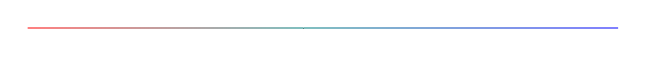
\begin{tikzpicture}
	\fill [left color=red!50, right color=teal!50] (0,0) rectangle (3.5,.01);
	\fill [left color=teal!50, right color=blue!50] (3.5,0) rectangle (7.5,.01);
	\end{tikzpicture}
\vspace{0.5cm}	
	
\begin{theorem}[ PE en una BON]

Sea $\mathcal B=\{\vec i,\, \vec j\}	 \ \text{ con } \ |\vec i|=|\vec j|= 1 \ \text{ y } \ \vec i \, \perp \, \vec j$, es decir, una BON

\vspace{2mm}Y sean $ \vec u=(u_1,u_2) \ \text{ y } \ \vec v=(v_1,v_2)$ dos vectores expresados en $\mathcal B$, entonces:


$$ \subrayado{ \boxed{\ \boldsymbol{ \vec u \cdot \vec v = u_1v_1+u_2v_2 } 	\ } } \, ; \qquad \boxed{\ |\vec u|=\sqrt{u_1^2+u_2^2} \ }\, ; \qquad  \boxed{ \ \cos \theta=\dfrac{ u_1v_1+u_2v_2 }{\sqrt{u_1^2+u_2^2}\,\sqrt{v_1^2+v_2^2}} \ } $$
\end{theorem}

\underline{Demostración}:
$\qquad B=\{\vec i, \vec j\} \ BON: \qquad |\vec i|=|\vec j|=1 \ \wedge \ \vec i \, \perp \vec j \quad \Rightarrow \quad \vec i \cdot \vec j=0 \, ; \ \ \vec i \cdot \vec i=\vec j \cdot \vec j=1$

$\triangleright \quad \vec u \cdot \vec v = (u_1,u_2)\cdot (v_1,v_2)=(u_1\, \vec i +u_2 \, \vec j)\cdot (v_1\, \vec i+v_2\, \vec j)=$

$\qquad \qquad = u_1v_1 \, \cancelto{1}{\vec i \cdot \vec i}+  u_1v_2 \, \cancelto{0}{\vec i \cdot \vec j}+   u_2v_1 \, \cancelto{0}{\vec j \cdot \vec i} +  u_1v_2 \, \cancelto{1}{\vec j \cdot \vec j} = u_1v_1+u_2v_2$ \QED

$\triangleright \quad \vec u \cdot \vec u = |\vec u|\, |\vec u|\, \cancelto{1}{\cos 0^o}  =|\vec u|^2= (u_1,u_2)\cdot (u_1,u_2)=(u_1\, \vec i +u_2 \, \vec j)\cdot (u_1\, \vec i+u_2\, \vec j)=$

$\qquad \qquad = u_1u_1 \, \cancelto{1}{\vec i \cdot \vec i}+  u_1u_2 \, \cancelto{0}{\vec i \cdot \vec j}+   u_2u_1 \, \cancelto{0}{\vec j \cdot \vec i} +  u_1u_2 \, \cancelto{1}{\vec j \cdot \vec j} = u_1^2+u_2^2 \ \to \ $ 

$\qquad \qquad  \to \ |u|\ = \ \sqrt{u_1^2+u_2^2} $\QED

$\triangleright \quad \vec u \cdot \vec v = |\vec u|\, |\vec v| \, \cos \theta \quad \to  \quad  \cos \theta=\dfrac{ u_1v_1+u_2v_2 }{\sqrt{u_1^2+u_2^2}\,\sqrt{v_1^2+v_2^2}} $\QED

\vspace{4mm}
\begin{theorem}

Dado un vector $\vec u=(u_1,u_2)$ expresado en una BON, un vector ortogonal (perpendicular) a él es 	$\vec u_\perp=(-u_2,u_1)\ $ \textcolor{gris}{(el vector $(u_2,-u_1)$ también es perpendicular a $\vec u$)} 
\end{theorem}
\underline{Demostración}: $\quad (-u_2,u_1)\cdot (u_1,u_2)=-u_1u_2+u_1u_2=0 \ \to \ (-u_2,u_1)\, \perp \,  (u_1,u_2)$\QED

\vspace{4mm}
\begin{miejercicio}	

Sean $\vec u=(3,-4)$ y $\vec v=(-1,3)$ dos vectores en una BON. Se pide:

\vspace{2mm} $a)\quad |\vec u|,\ \ |\vec v|,\ \ \theta=\measuredangle(\vec u, \vec v) $ 

$b)\ $ Determinar el valor de $k$ para que el vector $(4,k)$ sea perpendicular a $\vec v$

$c)\ $ Determinar un vector perpendicular a $\vec u$ y de módulo $10$

$d)\ $ Determinar un vector ortonormal (perpendicular y unitario) a $\vec v $

\rule{250pt}{0.1pt}

\vspace{2mm} $	\triangleright \ \ a)\quad  \ |\vec u|=\sqrt{3^2+(-4)^2}=5;\quad |\vec v|=\sqrt{(-1)^2+3^2}=\sqrt{10};$

\vspace{2mm}$ \cos \theta=\dfrac{3(-1)+(-4)3}{5\, \sqrt{10}}=\dfrac{-15}{5\sqrt{10}}=-\dfrac{3}{\sqrt{10}} \ \to \ \theta=18.4^o$

\vspace{4mm} $	\triangleright \ \ b)\quad (4,k)\cdot (-1,3)=-4+3k=0 \ \leftrightarrow \ k=\dfrac 4 3 $

\vspace{4mm} $	\triangleright \ \ c)\quad  \vec u=(3,-4)\ \to \ \vec u_\perp =(4,3);\ \ |\vec u_\perp|=\sqrt{4^2+3^2}=5 \ \Rightarrow \ $ 

\vspace{2mm} $\Rightarrow \ \ $ el vector pedido será $\ \vec w=2\vec u_\perp=2(4,3)=(8,6)$

\vspace{4mm} $	\triangleright \ \ d)\quad  \vec v=(-1,3) \ \to \ \vec v_\perp=(3,1);\ \ |\vec v_\perp|=\sqrt{3^2+1^2}=\sqrt{10} \ \Rightarrow \ $ 

\vspace{2mm} $\Rightarrow \ \ $ el vector pedido será $\ \vec w'=\dfrac{1}{\sqrt{10}}\, (3,1) = \left( \dfrac{3}{\sqrt{10}} , \dfrac{1}{\sqrt{10}} \right)$

	
\end{miejercicio}


\vspace{5mm} \textcolor{red}{Mientras no se diga lo contrario, se sobreentenderá que los vectores con los que vamos a tratar están expresados en una base ortonormal}	
	





%*****
\begin{miejercicio}	

Da un vector paralelo y uno perpendicular a los siguientes vectores:

$\vec u_1=(0,3);\qquad \vec u_2=(-4,0);\qquad \vec u_3=(12,-5);\qquad \vec u_4=(-2,-3)$

\rule{250pt}{0.1pt}

\vspace{2mm} Hay infinitas soluciones, daremos una de ellas en cada caso,

\vspace{2mm} $\vec u_{1\, \parallel}=(0,1);\qquad  \quad \ \vec u_{1\, \perp} =(-7,0)$
$\qquad \qquad \vec u_{2\, \parallel}=(1,0);\qquad  \vec u_{2\, \perp} =(1,4)$

\vspace{2mm} $\vec u_{3\, \parallel}=(-3,5/3);\qquad  \vec u_{3\, \perp} =(5,12)$
$\qquad \qquad \vec u_{4\, \parallel}=(2,3);\qquad  \vec u_{4\, \perp} =(3,-2)$

	
\end{miejercicio}


%*****
\begin{miejercicio}	

Dados $\vec u=(3,5)$ y $\vec v=(-1,3)$, calcula:

\begin{enumerate}[a) ]
\item $|\vec u|,\ \ |\vec v|,\ \ |\vec u-\vec v|,\ \ |\vec u+\vec v|$
\item $\vec u \cdot \vec v \ $ ;  Proy$_{\vec u}\vec v	\ $ y $\ \theta=\measuredangle (\vec u, \vec v)$
\item Un vector paralelo $\vec w_1$, a  $\vec u$ y de módulo $3$.
\item Un vector perpendicular $\vec w_2$ a $\vec v$ y unitario.
\item Un vector $\vec w_3$ del mismo sentido que $\vec u$ y sentido opuesto. 
\end{enumerate}
	

\rule{250pt}{0.1pt}

\vspace{2mm} $\triangleright \ \ a) \quad |\vec u|=\sqrt{3^2+5^2}=\sqrt{34};\qquad |\vec v|=\sqrt{(-1)^2+3^2}=\sqrt{10}$

\vspace{2mm} $\vec u+\vec v=(2,8) \ \to \ |\vec u+\vec v|=\sqrt{2^2+8^2}=\sqrt{68};\qquad 
\vec u-\vec v=(4,2) \ \to \ |\vec u+\vec v|=\sqrt{4^2+2^2}=\sqrt{20}$

\vspace{4mm} $\triangleright \ \ b) \quad \vec u \cdot \vec v=3\cdot(-1)+5\cdot 3=-3+15=12; \qquad Proy_{\vec u}\vec v=\dfrac{\vec u \cdot \vec v}{|\vec u|}=\dfrac{12}{\sqrt{34}} ; $

\vspace{2mm} $ \cos \theta=\dfrac{\vec u\cdot \vec v}{|\vec u|\,|\vec v|}=\dfrac{12}{\sqrt{34}\, \sqrt{10}} \ \to \ \theta=43.4^o$

\vspace{4mm} $\triangleright \ \ c) \quad \vec u=(3,5)\ $ tiene módulo $\sqrt{34}$; el vector $\dfrac 1{\sqrt{34}}\, (3,5)\ $ tiene módulo 1, luego, 

\vspace{2mm} $\vec w_1=3\, \dfrac 1{\sqrt{34}}\, (3,5)\ $ tendrá módulo 3 (compruébese). \textcolor{gris}{También lo es $\ -3\, \dfrac 1{\sqrt{34}}\, (3,5)$}

\vspace{4mm} $\triangleright \ \ d) \quad $ el vector $(3,1)$ es perpendicular a $\vec v$, que tiene por módulo $\sqrt{10}$, luego

\vspace{2mm} $\vec w_2 = \dfrac{1}{\sqrt{10}}\, (3,1) $ es perpendicular a $\vec v$ y unitario (módulo unidad) \textcolor{gris}{ó $\ -\dfrac{1}{\sqrt{10}}\, (3,1)$}

\vspace{4mm} $\triangleright \ \ e) \quad $ vectores paralelos a $\vec u$ son todos los de la forma $\ k\, \vec u=(3k,5k)$. Para que sean antiparalelos (sentido contrario), bastará multiplicar al $\vec u$ por un número negativo, 

\vspace{2mm} por ejemplo, $\quad \vec w_3=-2(3,5)=(-6,-10)$


	
\end{miejercicio}

%*****
\begin{miejercicio}	

Sea $\vec u=(-2,4)$, encuéntrese un vector $\vec v$ de módulo $\sqrt
{5}$ que forme $60^o$ con $\vec u$

\rule{250pt}{0.1pt}

\vspace{2mm} Sea $\ \vec v=(x,y) \ \to \ |\vec v|= \sqrt{5} = \sqrt{x^2+y^2}  \ \to \ x^2+y^2=5\quad (1*)$

\vspace{2mm} $\vec u \vdot \vec v=|\vec u|\, |\vec v|\, \cos \theta \ \to \ -2x+4y=\sqrt 5 \, \sqrt{(-2)^2+4^2}\, \cos 60 = \sqrt{5}\, \sqrt{20}\, \dfrac 1 2 \ \to \ -2x+4y=5\quad (2*)$

\vspace{2mm} $\begin{cases} \ -2x+y&=5 \quad (1*) \\ \ x^2+y^2&=5 \quad (2*)  \end{cases} \qquad \Rightarrow \quad  \vec v_1=\left( \dfrac{2\sqrt{3}-1}{2}\, , \,  \dfrac{2+\sqrt{3}}{2} \right) \qquad  \ \vec v_2=\left( -\dfrac{2\sqrt{3}+1}{2}\, ,\,\dfrac{2-\sqrt{3}}{2}\right)$

\begin{figure}[H]
	\centering
	\includegraphics[width=0.35\textwidth]{img-vec/vec15.png}	
\end{figure}

\end{miejercicio}


%*****

	





\newpage

\section{Ejercicios}


\begin{tikzpicture}
	\fill [left color=red!50, right color=teal!50] (0,0) rectangle (3.5,.1);
	\fill [left color=teal!50, right color=blue!50] (3.5,0) rectangle (7.5,.1);
	\end{tikzpicture}
\vspace{0.5cm}



\begin{mipropuesto}

Encuentra las componentes de $\vec w$ en la base $\mathcal B=\{\vec u_1,\vec u_2\}$ y en la base $\mathcal B'=\{\vec v_1,\vec v_2\}$	

	\begin{figure}[H]
	\centering
	\includegraphics[width=0.7\textwidth]{img-vec/vec17.png}	
\end{figure}
\end{mipropuesto}

\vspace{-8mm}
\begin{flushright}
\begin{footnotesize} \textcolor{gris}{\rotatebox{180}{ $\vec w=(2,-2)_{\mathcal B}= (2,1)_{\mathcal B'}$ }}	\end{footnotesize}
\end{flushright}





%%%%%%%%%%%%%%
\begin{mipropuesto}

\begin{multicols}{2}
La figura ABCD es un rombo de lado 6 cm y ángulos $60^o$ y $120^o$. Halla:

\vspace{6mm} $a) \ \ \overrightarrow{AB} \cdot \overrightarrow{AD}; \qquad  b) \ \ \overrightarrow{DA} \cdot \overrightarrow{DC};$

\vspace{4mm} $c)\ \  \overrightarrow{OB}\cdot \overrightarrow{OC};\qquad  d)\ \  \overrightarrow{AO} \cdot \overrightarrow{OC}$	
\begin{figure}[H]
	\centering
	\includegraphics[width=0.2\textwidth]{img-vec/vec16.png}	
\end{figure}
\end{multicols}
\end{mipropuesto}

\vspace{-8mm}
\begin{flushright}
\begin{footnotesize} \textcolor{gris}{\rotatebox{180}{ -18, 18, 0, 9 }}	\end{footnotesize}
\end{flushright}


%%%%%%%%%%%%%%
\begin{mipropuesto}

Dados los vectores $\vec a=(3, –2), \ \vec b=(–1, 2) \ \text{ y } \ \vec c=(0, –5)$, calcula $m$ y $n$ de modo que: $\ \vec c = m\vec a + n\vec b$.

\end{mipropuesto}

\vspace{-8mm}
\begin{flushright}
\begin{footnotesize} \textcolor{gris}{\rotatebox{180}{ m=-5/4, n=-15/4 }}	\end{footnotesize}
\end{flushright}



%%%%%%%%%%%%%%
\begin{mipropuesto}

Expresa el vector $\vec a =(–1, –8)$ como combinación lineal de $\vec b =(3, –2)$ y  $\vec c =(4, – 1/2)$	
\end{mipropuesto}

\vspace{-8mm}
\begin{flushright}
\begin{footnotesize} \textcolor{gris}{\rotatebox{180}{ $\vec a = 5\vec b - 4\vec c$ }}	\end{footnotesize}
\end{flushright}


%%%%%%%%%%%%%%
\begin{mipropuesto}

En una base ortonormal las coordenadas de un vector son $\vec v =(2, –5)$. Halla las coordenadas de $\vec v$ en la base $\mathcal B = \{(1, –1), (0, –1)\}$
\end{mipropuesto}

\vspace{-8mm}
\begin{flushright}
\begin{footnotesize} \textcolor{gris}{\rotatebox{180}{ $\vec v=(2,3)_{\mathcal B}$ }}	\end{footnotesize}
\end{flushright}

%%%%%%%%%%%%%%


\begin{mipropuesto}

Si A, B y C son los vértices de un triángulo equilátero de lado 1, calcula: 

\vspace{2mm}$ \overrightarrow{AB} \cdot \overrightarrow{AC};\quad 2 \overrightarrow{AB} \cdot  (-3 \overrightarrow{AC} );\quad  (\overrightarrow{AB} + \overrightarrow{AC})\cdot \overrightarrow{AB};\quad (2\overrightarrow{AB}-3\overrightarrow{AC})\cdot \overrightarrow{AC}$
\end{mipropuesto}

\vspace{-8mm}
\begin{flushright}
\begin{footnotesize} \textcolor{gris}{\rotatebox{180}{ 1/2, 3, 3/2, -2 }}	\end{footnotesize}
\end{flushright}




%%%%%%%%%%%%%%
\begin{mipropuesto}

Dados los vectores $\vec v_1=(-3,4)$ y $\vec v_2=(5,-1)$, calcular el producto escalar, sus módulos y el ángulo que forman (se supone, como siempre, que los vectores están expresados en una BON).
\end{mipropuesto}

\vspace{-8mm}
\begin{flushright}
\begin{footnotesize} \textcolor{gris}{\rotatebox{180}{ $-19,\ 5,\ \sqrt{26},\ 139.2^o$ }}	\end{footnotesize}
\end{flushright}

%%%%%%%%%%%%%%
\begin{mipropuesto}

Dado el vector $\vec v=(-5,3)$, calcula las coordenadas de los siguientes vectores (da todos las soluciones):
a) unitarios y de la misma dirección y sentido que $\vec v$
b) ortogonales a $\vec v$ y del mismo módulo
c) ortonormales a v	
d) ortogonales a $\vec v$
\end{mipropuesto}

\vspace{-8mm}
\begin{flushright}
\begin{footnotesize} \textcolor{gris}{\rotatebox{180}{ $a)\ (-5/\sqrt{34},3/\sqrt{34}) ,\quad b)\ \pm(3,5),\quad c)\ \pm (3/\sqrt{34},5/\sqrt{34}),\quad d)\ k(3,5)\, , \ \forall  k\neq 0 $}}	\end{footnotesize}
\end{flushright}

%%%%%%%%%%%%%%
\begin{mipropuesto}

Dados los vectores $\vec a$ y $\vec b$ tales que $|\vec a| = 3$, $|\vec b| = 2$ y el ángulo que forman es de $30^o$,  halla $| \vec a−\vec b|$ y $|\vec a+\vec b|$.	
\end{mipropuesto}

\vspace{-8mm}
\begin{flushright}
\begin{footnotesize} \textcolor{gris}{\rotatebox{180}{ 1.62 y 4.84 }}	\end{footnotesize}
\end{flushright}

%%%%%%%%%%%%%%
\begin{mipropuesto}

 Sabiendo que $|\vec u| = 3$ y $\vec u = -5\vec v$. Calcular $\vec u \cdot \vec v$	
\end{mipropuesto}

\vspace{-8mm}
\begin{flushright}
\begin{footnotesize} \textcolor{gris}{\rotatebox{180}{ $\theta=\measuredangle(\vec u, \vec v)=180^0, \qquad$ sol, -9/5 }}	\end{footnotesize}
\end{flushright}

%%%%%%%%%%%%%%
\begin{mipropuesto}

Encuentra un vector $\vec v$, de módulo 2, ortogonal a $\vec u=(21, 2)$	
\end{mipropuesto}

\vspace{-8mm}
\begin{flushright}
\begin{footnotesize} \textcolor{gris}{\rotatebox{180}{ $\pm \frac{\sqrt{5}}{5}\, (4,2)$ }}	\end{footnotesize}
\end{flushright}



%%%%%%%%%%%%%%
\begin{mipropuesto}

Dados los vectores $\vec u(1,-2), \ \vec v(3, 1) \ \text { y} \ \vec w(2, 0)$,

\vspace{2mm} a) calcula las coordenadas del vector $2\vec u - \vec v +\frac 1 3 \vec  w$

b) expresa $\vec w$ como combinación lineal de $\vec u$ y $\vec v$

c) calcula los ángulos que forman dos a dos

d) halla un vector con la misma dirección que $\vec u$ y de módulo $\sqrt{20}$

e) halla un vector unitario y perpendicular a $\vec v$.	
\end{mipropuesto}


\vspace{-8mm}
\begin{flushright}
\begin{footnotesize} \textcolor{gris}{\rotatebox{180}{ $a)\ \ (-1/3,-5);\quad b)\ \ \vec w=2/7 \vec u + 4/7 \vec v;\quad c) \ \ 81.9^o, \ 63.4^o,\ 18.4^o; \quad d)\ \ \pm(2,-4);\quad e)\ \ \pm \sqrt{10}/10 \, (1,-3)$ }}	\end{footnotesize}
\end{flushright}


%%%%%%%%%%%%%%
\begin{mipropuesto}

Dados los vectores $\vec u=(1, 2)$ y $\vec v=(-3, 1)$:

\vspace{2mm} a) Comprueba que $\vec u$ y $\vec v$ forman una base.

b) Encuentra las componentes del vector $\vec w =(-1, 5)$ en la base $\mathcal B = \{ \vec u,\, \vec  v \}$
\end{mipropuesto}

\vspace{-8mm}
\begin{flushright}
\begin{footnotesize} \textcolor{gris}{\rotatebox{180}{ $a)\ \ \vec u \ \not \parallel \ \vec v ;\qquad b)\ \ \vec w=(2,1)_{\mathcal B}=2\vec u+\vec v$}}	\end{footnotesize}
\end{flushright}


%%%%%%%%%%%%%%
\begin{mipropuesto}

Si $\vec u=(2, k)$ y $\vec v(1, -4)$ determina el valor de k para que: 

\begin{multicols}{2} a) $\vec u$ y $\vec v$ sean perpendiculares

c) $\vec u \cdot \vec v=10$	

b) $\vec u$ y $\vec v$ tengan el mismo módulo

d)  $\vec u$ y $\vec v$  formen $45^o$ \end{multicols}
\end{mipropuesto}

\vspace{-8mm}
\begin{flushright}
\begin{footnotesize} \textcolor{gris}{\rotatebox{180}{ $a)\ \ k=1/2;\qquad b)\ \ k=\pm \sqrt{13};\qquad c)\ \ k=-2;\qquad d)\ \ k=2(\sqrt{87}-16)/13 \ \vee \ k=-2(\sqrt{87}+16)/13$ }}	\end{footnotesize}
\end{flushright}


%%%%%%%%%%%%%%
\begin{mipropuesto}

Dada la base $\mathcal B = \{ \vec u, \vec v\}$,  donde $\vec u=(3, –4)$ y $\vec v=(0, –8)$, determina, en cada caso, una base $\mathcal B'$ de vectores unitarios tales que:

\vspace{2mm} 
a) Los vectores de $\mathcal B'$ sean paralelos a los de $\mathcal B$.

b) Los vectores de $\mathcal B'$ sean perpendiculares a los de $\mathcal B'$ 	
\end{mipropuesto}

\vspace{-8mm}
\begin{flushright}
\begin{footnotesize} \textcolor{gris}{\rotatebox{180}{ $a)\ \mathcal B'=\{(3,5/-4/5),\ (0,-1)\};\qquad b)\  \mathcal B'=\{(4,3), \ (8,0)\}$}}	\end{footnotesize}
\end{flushright}


%%%%%%%%%%%%%%
\begin{mipropuesto}

Dados $\vec u=(1/2,k)$ y $\vec v=(1/2,0)$, calcula $k$ para que $\vec u$ y $\vec v$ formen un ángulo de $60^o$	
\end{mipropuesto}

\vspace{-8mm}
\begin{flushright}
\begin{footnotesize} \textcolor{gris}{\rotatebox{180}{ $k=\pm \sqrt{3}/2$ }}	\end{footnotesize}
\end{flushright}


%%%%%%%%%%%%%%
\begin{mipropuesto}

Dados los vectores $\vec u= (–1, a)$ y $\vec v= (b, 15)$, halla $a$ y $b$, en cada caso, de modo que: $\ a)\  \vec u \perp  \vec v \ $  y $\ |\vec u| = 10$ $\quad b)\  \vec u \cdot  \vec v = 7 \ $ y $\ |\vec  v | = 17$	
\end{mipropuesto}

\vspace{-8mm}
\begin{flushright}
\begin{footnotesize} \textcolor{gris}{\rotatebox{180}{ $a)\ \ a=3,\ b=45;\qquad b)\ \ a=1,\ b=8 $ }}	\end{footnotesize}
\end{flushright}


%%%%%%%%%%%%%%
\begin{mipropuesto}

Dados los vectores $\vec a = 2 \vec u - \vec v$ y $\vec b = –3 \vec u + k \vec v$ , siendo $\vec u = (2, 3)$ y $\vec v = (-3, 0)$, halla $k$ de modo que $(\vec a + \vec b)$ ) sea ortogonal a $(\vec a - \vec b)$	
\end{mipropuesto}

\vspace{-8mm}
\begin{flushright}
\begin{footnotesize} \textcolor{gris}{\rotatebox{180}{ $k=-4/3 \ \vee \ k=-8/3$ }}	\end{footnotesize}
\end{flushright}


%%%%%%%%%%%%%%
\begin{mipropuesto}

Halla un vector unitario que forme un ángulo de $30^o$ con el vector $\vec u= (1, \sqrt{3} )$
	
\end{mipropuesto}

\vspace{-8mm}
\begin{flushright}
\begin{footnotesize} \textcolor{gris}{\rotatebox{180}{ $(0,1) \ \vee \ \frac 1 2(\sqrt{3},1)$ }}	\end{footnotesize}
\end{flushright}


%%%%%%%%%%%%%%
\begin{mipropuesto}

Obtén un vector $\vec u=(x, y)$ ortogonal a $\vec v=(8, 6)$ y cuyo módulo sea la mitad del de $\vec v$.	
\end{mipropuesto}

\vspace{-8mm}
\begin{flushright}
\begin{footnotesize} \textcolor{gris}{\rotatebox{180}{ $\pm(3,-4)$ }}	\end{footnotesize}
\end{flushright}

\vspace{10mm}

\begin{myexampleblock}{Vectores 3-D}

\vspace{3mm} 

\begin{multicols}{3}
\begin{figure}[H]
	\centering
	\includegraphics[width=0.3\textwidth]{img-vec/vec21.png}	
\end{figure}

\begin{figure}[H]
	\centering
	\includegraphics[width=0.25\textwidth]{img-vec/vec22.png}	
\end{figure}

\begin{figure}[H]
	\centering
	\includegraphics[width=0.3\textwidth]{img-vec/vec23.png}	
\end{figure}	
\end{multicols}

\vspace{3mm}

\end{myexampleblock}





%++++++++++++++++++++++++++++++++++++
%********************************************************************
\newpage
%\vspace{3cm} %%%%%%%%%%%%%%%%%%%%%%%
\begin{adjustwidth}{50pt}{250pt}
\begin{cuadro-naranja}
\textbf{\huge{Problemas $\boldsymbol{+}$}}\normalsize{$\, $}
\end{cuadro-naranja}	
\end{adjustwidth}

\vspace{5mm}
\begin{enumerate}[\textbf{P$\boldsymbol +$} 1. ]


%%%%
\item	Considera el vector $\vec u=(\cos \theta,-\sin \theta)$, ?`es unitario? Determina un vector ortonormal a $\vec u$, ?`hay solo uno?

\vspace{-6mm}
\begin{flushright}
\begin{footnotesize} \textcolor{gris}{\rotatebox{180}{ Sí, $\vec v=(\sin \theta,\cos \theta) \, \perp \, \vec u$, no ($-\vec v $ también lo es) }}	\end{footnotesize}
\end{flushright}


%%%%
\item	Probar, con un contraejemplo, que $\ \vec u \cdot \vec w = \vec v \cdot \vec w \ \ \not \Rightarrow \ \ \vec u = \vec v$

\vspace{-6mm}
\begin{flushright}
\begin{footnotesize} \textcolor{gris}{\rotatebox{180}{ $\vec u=(3,2),\ \vec v= (1,4),\ \vec w= (1,1)$ }}	\end{footnotesize}
\end{flushright}


%%%%
\item	Sabiendo que $|\vec u|=4$ y que $\dfrac{\vec u}{\vec v}=\dfrac 3 2 $, determina $\ \vec u \cdot \vec v$

\vspace{-6mm}
\begin{flushright}
\begin{footnotesize} \textcolor{gris}{\rotatebox{180}{ $\vec u$ misma dirección y sentido que $\vec v$, ya que $\vec u=\frac 3 2 \vec v$. El resultado es $\vec u \cdot \vec v=32/3$ }}	\end{footnotesize}
\end{flushright}


%%%%
\item	Si $\vec u$ y $\vec v$ son vectores ortogonales y de módulo 1, hallar los posibles valores del parámetro real $\alpha$ para que los vectores $\vec u+\alpha \vec v$ y $\vec u-\alpha \vec v$ formen un ángulo de $60^o$

\vspace{-6mm}
\begin{flushright}
\begin{footnotesize} \textcolor{gris}{\rotatebox{180}{ $\alpha=\pm \sqrt{3}/3$ }}	\end{footnotesize}
\end{flushright}




%%%%
\item	Sean A, B y C los vértices de un triángulo. Si $\overrightarrow{AB}= (–1, 4), \ \overrightarrow{AC}= (3, –1) \ \text{ y } \ \overrightarrow{BC}= (4, –5)$, ?`puede tratarse de un triángulo rectángulo?

\vspace{-6mm}
\begin{flushright}
\begin{footnotesize} \textcolor{gris}{\rotatebox{180}{ No, $\ (\overrightarrow{AB}\cdot \overrightarrow{AC} \neq 0, \ \ \overrightarrow{BA}\cdot \overrightarrow{BC} \neq 0;\ \ \overrightarrow{CA}\cdot \overrightarrow{BC} \neq 0)$ }}	\end{footnotesize}
\end{flushright}



%%%%
\item	Sea $\mathcal B=\{\vec x, \, \vec y\}$ una base ortonormal. Calcula $\ |\vec x + \vec y|$  y $|\vec x – \vec y|$

\vspace{-6mm}
\begin{flushright}
\begin{footnotesize} \textcolor{gris}{\rotatebox{180}{ $\sqrt{2}$ en ambos casos }}	\end{footnotesize}
\end{flushright}


%%%%
\item	Halla un vector $\vec u$ que forme un ángulo de $60^o$ con el vector $\vec v=(2, 2 \sqrt{3})$ y tenga como módulo la mitad del módulo de $\vec v$.

\vspace{-6mm}
\begin{flushright}
\begin{footnotesize} \textcolor{gris}{\rotatebox{180}{ $(–1, \sqrt{3}) \ \vee \   (2, 0) $ }}	\end{footnotesize}
\end{flushright}


%%%%
\item	De una base $\mathcal B = \{ \vec u, \vec v\}$ se sabe que $|\vec u| = 2, \ |\vec v| = 1 \ \text{ y } \  \vec u \cdot \vec  v = –1$. En esa base las coordenadas de dos vectores son $\vec x(=1, 2) \ \text{ e } \  \vec y=(–1, 1)$. Calcula $\vec x \cdot \vec y$

\vspace{-6mm}
\begin{flushright}
\begin{footnotesize} \textcolor{gris}{\rotatebox{180}{ Expresa $\vec x \ \text{ y } \  \vec y$ en función de $ \vec u \ \text{ y } \  \vec v\}$ y aplica la definición de producto escalar. Sol: 7}}	\end{footnotesize}
\end{flushright}




%%%%
\item	Se sabe que $\vec c = \vec a + 2\vec b$ y $\vec d = 5\vec a - 4\vec b$ son perpendiculares y que $\vec a$ y $\vec b$ son unitarios. ?`Cuál es el ángulo que forman $\vec a$ y $\vec b$?

\vspace{-6mm}
\begin{flushright}
\begin{footnotesize} \textcolor{gris}{\rotatebox{180}{ $120^o$ }}	\end{footnotesize}
\end{flushright}

%%%%
\item	Demuestra que el vector $(\vec b \cdot \vec c) \, \vec a - (\vec a \cdot \vec c)\, \vec b$ es perpendicular al vector $\vec c$.

\vspace{-6mm}
\begin{flushright}
\begin{footnotesize} \textcolor{gris}{\rotatebox{180}{ Trabaja en componentes y comprueba qu el producto escalar e cero $\quad (\, \vec a=(a_1,a_2),\ \vec b=(b_1,b_2),\ \vec c=(c_1,c_2) \, )$ }}	\end{footnotesize}
\end{flushright}

%%%%
\item	Una barca se desplaza por un río en dirección sur a una velocidad de 20 km/h. Si empieza a soplar un viento en dirección este a 5 km/h, ?en qué dirección y a qué velocidad se moverá la barca?

\vspace{-6mm}
\begin{flushright}
\begin{footnotesize} \textcolor{gris}{\rotatebox{180}{ $14.1^o$ }}	\end{footnotesize}
\end{flushright}


%%%%
\item	Justifica por qué $\ |\vec  a \cdot \vec b | \ \leqslant \  | \vec a | \,  | \vec b |$

\vspace{-6mm}
\begin{flushright}
\begin{footnotesize} \textcolor{gris}{\rotatebox{180}{ Calcula el producto escalar y ten en cuenta que el coseno de un ángulo siempre es menor o igual que uno.  }}	\end{footnotesize}
\end{flushright}



\end{enumerate}






\newpage
\section{Resumen del tema}

\begin{tikzpicture}
	\fill [left color=red!50, right color=teal!50] (0,0) rectangle (3.5,.1);
	\fill [left color=teal!50, right color=blue!50] (3.5,0) rectangle (7.5,.1);
	\end{tikzpicture}
\vspace{1.5cm}	
	
	
\begin{myblock}{Resumen \emph{``Vectores''}}

\vspace{2mm}
$$k\, (u_1,u_2) \ = \ (ku_1,ku_2)\qquad \qquad (u_1,u_2)\ + \ (v_1,v:2)\ = \ (u_1+v_1,u_2+v_2)$$

$$\boldsymbol{ \vec u \cdot \vec u \ = \ |\vec u|\ |\vec v|\ \cos \theta \ = \ u_1v_1 \, + \, u_2v_2}\, , \ \text{ en una BON} $$

$$|\vec u|\ = \ \sqrt{\, \vec u \cdot\, \vec u} \ = \ \sqrt{u_1^2+u_2^2}\, , \ \text{ en una BON} $$

$$\vec u \, \parallel \, \vec u \ \leftrightarrow \ \exists k \in \mathbb R \ / \ \vec u = k\, \vec v \ \leftrightarrow \ \dfrac{u_1}{v_1}=\dfrac{u_2}{v_2}$$

$$\vec u \, \perp \, \vec v \ \leftrightarrow \ \vec u \cdot \vec v \ = \ 0  \ \textcolor{gris}{ \leftrightarrow \ u_1v_1+u_2v_2=0 \, , \ \text{ en una BON} }$$
 
	
\end{myblock}
	
	
	
	

\begin{comment}

%%%%%%%%%%%%%%%%%%%%%%%%%%%%%%%%%%%. SECCIONES
\chapter{texto}

\begin{tikzpicture}
	\fill [left color=red!50, right color=teal!50] (0,0) rectangle (6.5,.2);
	\fill [left color=teal!50, right color=blue!50] (6.5,0) rectangle (11.5,.2);
	\end{tikzpicture}

\vspace{1cm}
\section{texto}

\begin{tikzpicture}
	\fill [left color=red!50, right color=teal!50] (0,0) rectangle (3.5,.1);
	\fill [left color=teal!50, right color=blue!50] (3.5,0) rectangle (7.5,.1);
	\end{tikzpicture}
\vspace{0.5cm}

\subsection{texto}
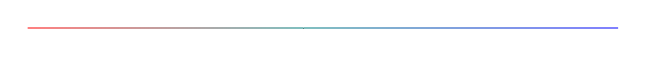
\begin{tikzpicture}
	\fill [left color=red!50, right color=teal!50] (0,0) rectangle (3.5,.01);
	\fill [left color=teal!50, right color=blue!50] (3.5,0) rectangle (7.5,.01);
	\end{tikzpicture}
\vspace{0.5cm}


%%%%%%%%%%%%%%%%%%%%%%%%%%%%%%%%%%%. \begin{ ------>. 
detsacado;  cuadro-naranja;  cuadro-gris;  miejercicio (solución extensa);  mipropuesto (solución corta y fuera del cuadro)

%%%%%%%%%%%%%%%%%%%%%%%%%%%%%%%%%%%. CURIOSIDAD
\vspace{1cm}
\color{ForestGreen!80}
\rule{250pt}{0.2pt}
Texto
\vspace{-8mm}
\begin{flushright}
\rule{250pt}{0.2pt}		
\end{flushright}	
\color{black}
\end{comment}